%----------------------------------------------------------------------------
\chapter{Tervezés és implementáció}
%----------------------------------------------------------------------------

\section{Tervezés, döntési lehetőségek értékelése}

\subsection{Python}

A Python napjaink egyik legelterjedtebb programozási nyelve. Egy könnyen programozható és átlátható, interpretált nyelv, melyben a megírt program kódot a Python értelmező sorról-sorra értelmezi és futtatja, nincs különválasztva a forrás és a fordított kód. Deep learning körökben is a Python nyelv dominál, rengeteg deep learning toolkit erre a nyelvre épít, így választásom a fejlesztéshez természetesen a Python nyelvre esett.

\subsection{NeMo}

A neurális hálók komplikáltságából adódik, hogy pontos és precíz implementációjuk igen bonyolult és időigényes. Emiatt célszerű a már meglévő, bejáratott és bizonyított lehetőségeket használni, így felgyorsítva a fejlesztési folyamatot. Több deep learing platform is található az internetet, mint például a Tensorflow vagy PyTorch. Az Nvidia által fejlesztett NeMo egy olyan összetett és folyamatosan karbantartott toolkit, melynek segítségével különböző mesterséges intelligencia alapú társalgási, beszéddel kapcsolatos applikációkat, alkalmazásokat készíthetünk.

% https://github.com/NVIDIA/NeMo

Az alap koncepcióját a toolkit-nek az úgynevezett Neurális Modulok alkotják. Ezek a modulok lehetnek például adat rétegek, kódolók, dekóderek, nyelv modellek vagy loss függvények. A modulok ereje abban rejlik hogy egymáshoz viszonyítva tetszőlegesen építhetők, cserélhetők, törölhetők. Egy egyszerű módosítással kicserélhető például a loss számításához használt függvény anélkül, hogy a kódot a többi modulban módosítani kéne.

Az 3.1-es táblán látható modellek közül az Nvidia fejlesztette a legkevésbé számításigényeset, mely figyelemreméltó eredményeket produkál. Ez a QuartzNet modell, ami az alacsony paraméterszáma ellenére SOTA eredményeket ér el. A felsorolt okokból kifolyólag a fejlesztési folyamat elvégzéséhez választásom a NeMo toolkit-re esett.

\subsubsection{PyTorch}

A NeMo a PyTorch nevű, Facebook-os kutatók által fejlesztett, mesterséges intelligencia fejlesztésére szakosodott nyílt forráskódú keretrendszerre épít. A PyTorch a TensorFlow-nál magasabb szintű, könnyebben kezelhető keretrendszer, mely egyre inkább elterjedtté válik a kutatók és fejlesztők körében.

\subsubsection{QuartzNet}

A kísérleteimet QuartzNet architektúrájú modellekkel tervezem elvégezni a korábban említett alacsony paraméterszáma és magas precizitása végett. Az architektúra (4.1-es ábra) nagyban hasonlít egy másik Nvidia által fejlesztett architektúrához, a Jasper-hez. A modell B darab blokkból áll. Egy opcionálisan beállítható dropout modul jelenhet meg a modellben, illetve CTC loss függvény számítás található benne. A már említett blokkok további, R darab blokkból állnak, melyek konvolúciós rétegekből, batch normalizálókból és ReLU aktivációs függvényből épülnek fel. Ezáltal a QuartzNet pontos felépítésére QuartzNet BxR alakban szokás hivatkozni. A legnagyobb Nvidia által készített a Quartznet 15x5, mely 18.9 millió paraméterből áll.

A QuartzNet a Jasper-től a konvolúciós rétegében tér el. A sima egy dimenziós konvolúciós réteg helyett, egy dimenziós idő-csatorna szerinti (time-channel separable) konvolúciós rétegeket használ. Ennek a fő tulajdonsága, hogy jóval kevesebb paramétert használ az eredeti koncepciónál. Ennek köszönhetően mélyebb hálókat lehet készíteni nagyobb konvolúciós filter-ekkel anélkül, hogy a a paraméterek száma, ezáltal a szükséges számítása kapacitás túlzottan megnövekedne.

% https://arxiv.org/abs/1910.10261

\begin{figure}[!ht]
\centering
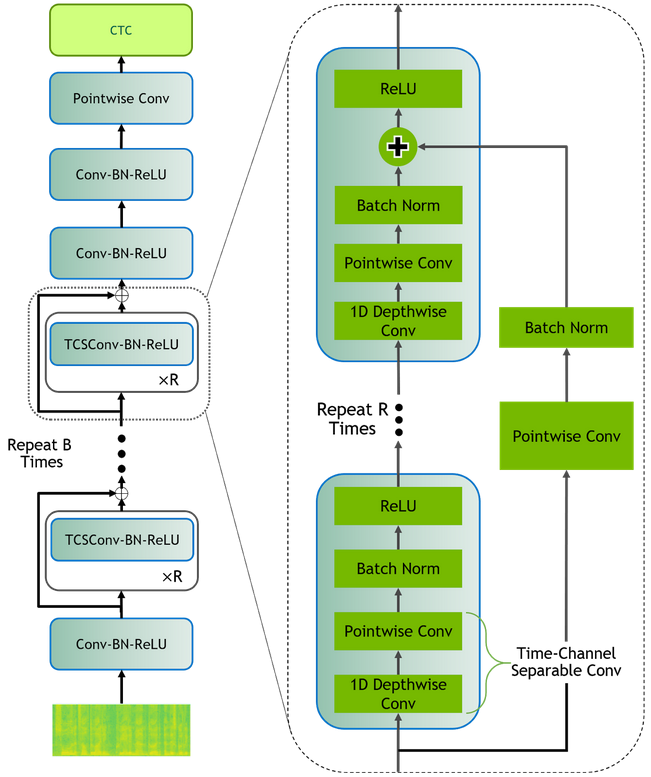
\includegraphics[width=150mm, keepaspectratio]{figures/QuartzNet-architecture.png}
\caption{QuartzNet architektúra.}
\label{fig:TeXstudio}
\end{figure}

% https://developer.nvidia.com/blog/develop-smaller-speech-recognition-models-with-nvidias-nemo-framework/

\subsection{TensorBoard}

Az eredmények kiértékeléséhez és nyomonkövetéséhez a TensorBoard-ot, a TensorFlow egy vizualizációs toolkit-jét használom. Több funkcióval is rendelkezik, mint például a súlyok időbeni változásának vizualizációja, illetve a tanítóadatok, képek, szöveg vagy hang anyag kijelzése. Számomra a legfontosabb tulajdonsága az egyes metrikák, a loss és a pontosság, WER, értékének változása.

% https://www.tensorflow.org/tensorboard

A TensorBoard könnyedén indítható a következő parancs kiadásával: $tensorboard --logdir ~/lightning-logs$ , ahol a logdir kapcsoló adja meg melyik könyvtárban keressen TensorBoard kompatibilis log-okat, event-eket. A szükséges event-ek előállítása könnyedén végezhető a NeMo toolkit segítségével, mely támogatja a megfelelő callback függvények használatát, amik az event-ek batch-enkénti frissítsét tesznek lehetővé.

\begin{figure}[!ht]
\centering
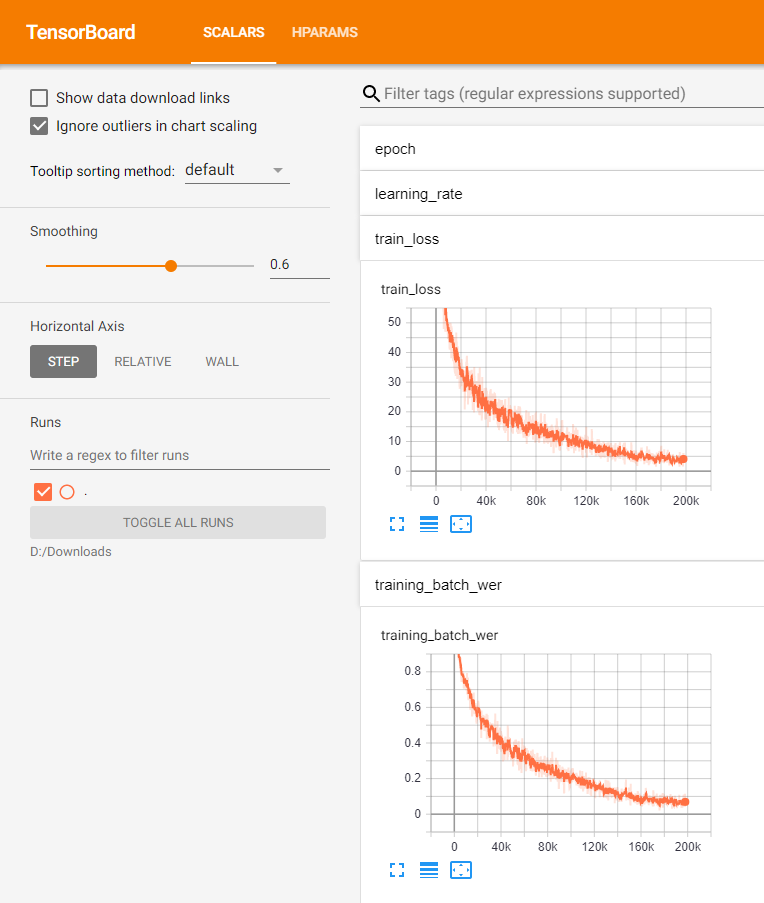
\includegraphics[width=150mm, keepaspectratio]{figures/tensorboard-example.png}
\caption{Lokálisan futtatott TensorBoard.}
\label{fig:TeXstudio}
\end{figure}

\section{Angol, majd orosz}

Kezdetben a tesztelést az egyik leggyakoribb nyelven, az angolon, végeztem. Ennek oka főként az, hogy megbizonyosodjak a modellem és a NeMo beállításainak sikerességéről, hogy megfelelő eredményeket tudok elérni elterjedt, kisebb adatbázisokon. Másfelől a modellem hiperparamétereit, mint például a learning rate, optimalizáltam, és az orosz nyelven történő kísérletezésnek a legbiztatóbb beállításokkal tudtam nekiállni.

Az angol nyelvű eredményeket viszonyításként is fel tudtam használni az végső orosz eredményekkel való összehasonlításánál, ahol a nagyságrendileg azonos mennyiségű orosz adatoknak az angoléhoz hasonló eredményeket produkálhattak.

\subsection{Google Colab}

A NeMo-val való ismerkedéshez felhasználtam az Nvidia által írt jupyter notebook-okat, melyeket könnyedén lehet az ingyenes használható Google Colab-ból futtatni. A Colab ingyenes hozzáférést nyújt GPU erőforrásokhoz, ahol egyenesen a böngészőből futtatható a Python kód és az eredményeket akár le is lehet tölteni.

Sajnos a Colab bizonyos órán belül felfüggeszti a munkamenetet, illetve a nagy mennyiségű adatok munkamenetenkénti le- és feltöltése időigényes. Ezért a rövidebb adatbázisokon, mint például az AN4-en, túl nem jelent a tesztelésen és toolkit-tel való ismerkedésen túl megoldást.

% https://github.com/NVIDIA/NeMo/blob/main/tutorials/asr/01_ASR_with_NeMo.ipynb
% Google Colab, https://colab.research.google.com/notebooks/intro.ipynb

\section{Adatbázisok}

A megfelelő modell megtalálásához két darab angol nyelvű adatbázist is használtam. Mikor elégedett voltam az eredményekkel és megbizonyosodtam, hogy sikeresen beállítottam a NeMo toolkit-et is, áttértem az orosz nyelvű modell fejlesztésére.

Az adatbázisokon belül szükséges három különböző típusú egymástól független adathalmazt megállapítani. Az egyik a tanító adathalmaz, ezeket a hanganyagokat közvetlen a háló tanítására használjuk. Fontos egy validációs vagy teszt adathalmaz is, amit tanítás közben használunk kiértékelésre, a tanítás általános pontosságának értékelésére. A harmadik dev adathalmaz pedig azért szükséges, mert a validációs adathalmaz pontosságát igyekszünk javítani, majd amikor ezzel elégedettek vagyunk egy tőle független adathalmazzal vizsgálhatjuk meg a végső pontosságot.

\subsection{Adatok előfeldolgozása}

Magukat a hangfájlokat is meg kell vizsgálni, egységesíteni kell a tanítás előtt. A leggyakrabban használt kiterjesztés a .wav, így én is ennek a használata mellett döntöttem. Szükség esetén az egyes hangfájlokat át kell konvertálni ebbe a formátumba a tanítás, kiértékelés előtt.

A hanganyagok mintavételezése sem elhanyagolható. Míg a túl alacsony mintavételezés minőségi romlást, ezáltal rosszabb eredményeket okozhat, a túl magas mintavételezés lassítja a tanítási folyamatot és akár szintén rosszabb eredményeket produkálhat.

Az adatbázisok esetén megvizsgálandó, hogy hány beszélő hangja található benne. Minél több van benne annál általánosabban alkalmazható jobb eredményekkel.

\subsection{AN4}

Az "AN4" vagy "census" angol nyelvű beszéd adatbázist 1991-ben vették fel a Carnegie Mellon Egyetemen. A különböző beszélők betűzve mondanak olyan adatokat mint születési dátum, telefonszám, név vagy egyéb véletlenszerűen generált, előre definiált kontroll szavakat.

% részletes infó: "Acoustical and environmental robustness in automatic speech recognition", by Alex Acero, published by Kluwer Academic Publishers, 1993
% http://www.speech.cs.cmu.edu/databases/an4/README.html

Az adatbázis két különböző részre van osztva, az első a tanítást szolgálja, míg a második része a tesztelést. Ez előbbi 50 percnyi beszédet tartalmaz, míg a tesztelésre szolgáló rész 6 percet. Rövidségéből adódóan gyorsan tanítható és értékelhető, mely ideálissá teszi gyors kalibrálási, beállítási feladatok megoldására.

\subsection{LibriSpeech}

A LibriSpeech egy több száz órát tartalmazó, szintén angol nyelű, hangos könyv gyűjtemény. Ez az egyik leginkább használt adatbázis, melyet előszeretettel alkalmaznak tudományos, kutatási anyagok eredményeinek ismertetésekor is.

Az elérhető hanganyag fele tiszta, könnyen érthető, míg másik fele zajosabb körülmények közt lett felvéve vagy kevésbé kivehető. Külön tartalmaz tanító, teszt és dev adathalmazokat.

\subsection{Mozilla Common Voice}

A Mozilla Common Voice egy Mozilla által indított projekt. Célja, hogy különböző nyelveken, így oroszul is, a közösség erejét felhasználva gyűjtsön anonim hanganyagokat. Bárki felveheti a saját hangját, előre meghatározott szövegeket felolvasva, illetve érvényesíthet mások által felolvasott szövegeket. A biztonság kedvéért egy szöveget két személynek is jóvá kell hagynia.

% https://voice.mozilla.org/

Orosz hangból durván 100 órányi áll rendelkezésre, de tüzetesebb vizsgálat után észrevettem, hogy ebből ~10-10 óra a teszt és dev adathalmaz mérete, míg ~20 óra a tanító adathalmazé. A maradék ~60 órából több azért nincs használva, mert megismételt szöveget olvasnak fel benne, vagy rövid hanganyagokat tartalmaz. A tanító adathalmazt sikerült feldúsítsam ~45 óra környékére azáltal, hogy belevettem a 100 órányi hangból az összes olyan hangot, melyek nem voltak benne sem a teszt sem a dev adathalmazokban.

% insert random data analysis here?

\subsection{További orosz adatbázisok}

Mivel a Mozilla Common Voice orosz nyelvű adatbázisa legfeljebb 45 órányi tanítóadattal rendelkezik, míg a LibriSpeech-é mely eredményeihez viszonyítani szeretnénk 100 órán lett tanítva, ezért több tanítóadatot is be kellett vonni. Egy ingyenesen hozzáférhető github-on található projektben több adatbázis is található, többnyire .opus formátumban. Elsősorban a radio2 adatbázissal dolgoztam.

Fontos nem elfelejteni a Mozzila Common Voice és egyéb rádión található hanganyagok közötti különbséget. Míg előbbi többnyire bediktált, felolvasott szöveget tartalmaz különböző minőségben és tempóban, utóbbi kötetlenebb, tisztább minőségű beszélgetéseket is tartalmazhat.

% radio_2 vs mozilla adatbázis összehasonlítás?

% https://github.com/snakers4/open_stt/blob/master/README.md

\section{NeMo beállítása}

A NeMo egy folyamatosan frissített, alaposan karbantartott toolkit, mely nemrég lépett 1.0.0 verzióra. A munkám során az 1.0.0b verzióval dolgoztam. 

\section{Kísérletek}